\documentclass[nobib]{MSword}
% Class options:
%-------------------------------
% nobib         - skip bibliography code/ don't include bib
% math          - include math packages and useful math commands
% hidelinks     - hide hyperref colored link boxes
% wordlinks     - link color scheme similar to word


% Preamble code:
%%%%%%%%%%%%%%%%%%%%%%%%%%%%%%%%%%%%%%%%
\usepackage[english]{babel}
\usepackage{csquotes}
\usepackage{lipsum}

% % Uncomment using "Ctrl + /" (/ on numpad):
% % Customizing headers and footers:
% \fancypagestyle{custom}{%
%     \fancyhf{}% clears the footer and header
%     % Header:
%     \fancyhead[L]{}
%     \fancyhead[C]{}
%     \fancyhead[R]{}
%     % Footer:
%     \fancyfoot[L]{}
%     \fancyfoot[C]{}
%     \fancyfoot[R]{}
%         % Tips:
%         % ----
%         % L: left, C: center, R: right
%         % O: odd pages, E: even pages
%         % ----
%         % Example: \fancyghead[LO,RE]{Text}
%         % will produce "Text" left in the header
%         % on odd pages and right in the header on even pages.
%     % Rules/ lines:
%     \renewcommand{\headrulewidth}{0.4pt}
%     \renewcommand{\footrulewidth}{2pt}
% }
% % Changing the pagestyle:
% \pagestyle{custom}

%%%%%%%%%%%%%%%%%%%%%%%%%%%%%%%%%%%%%%%%

% Preamble information:
%%%%%%%%%%%%%%%%%%%%%%%%%%%%%%%%%%%%%%%%

\title{Z - Transform Operations}
\author{Dre Mata}
\date{4 April 2023}

%%%%%%%%%%%%%%%%%%%%%%%%%%%%%%%%%%%%%%%%

% The document:
%%%%%%%%%%%%%%%%%%%%%%%%%%%%%%%%%%%%%%%%
\begin{document}

\maketitle
\begin{center}
    Part 1:
\end{center}
The objective of this lab is to gain familiarity of Python's built in functions and a function created by Christopher Felton to analyze a discrete system. the first task is to find the transfer function of the causal function seen below. 

\begin{center}
$ y[k] = 2x[k] - 40x[k-1] + 10y[k-1] -16y[k-2] $
\end{center}

The process for finding the transfer function can be seen in figure one. The second task was to find h[k] using partial fraction expansion. This can be seen in figure two. The third task was to use the scipy.signal.residuez() function to do the partial fraction expansion in python. The results of this can be seen in figure three. The next task was to use the zplane() function to plot the pole-zero for H(z). The plot for this can be seen in figure four. The next task was to use the scipy.signal.freqz() to plot the magnitude and phase response for H(z). These plots can be seen in figure five.

\begin{center}
    Questions:
\end{center}

1. Looking at the plot generated in Task 4, is H(z) stable? Explain why or why not.

The plot does appear to be stable, because there is not exponentially increasing line in it.

\begin{center}
    Figures
\end{center}

Figure 1:

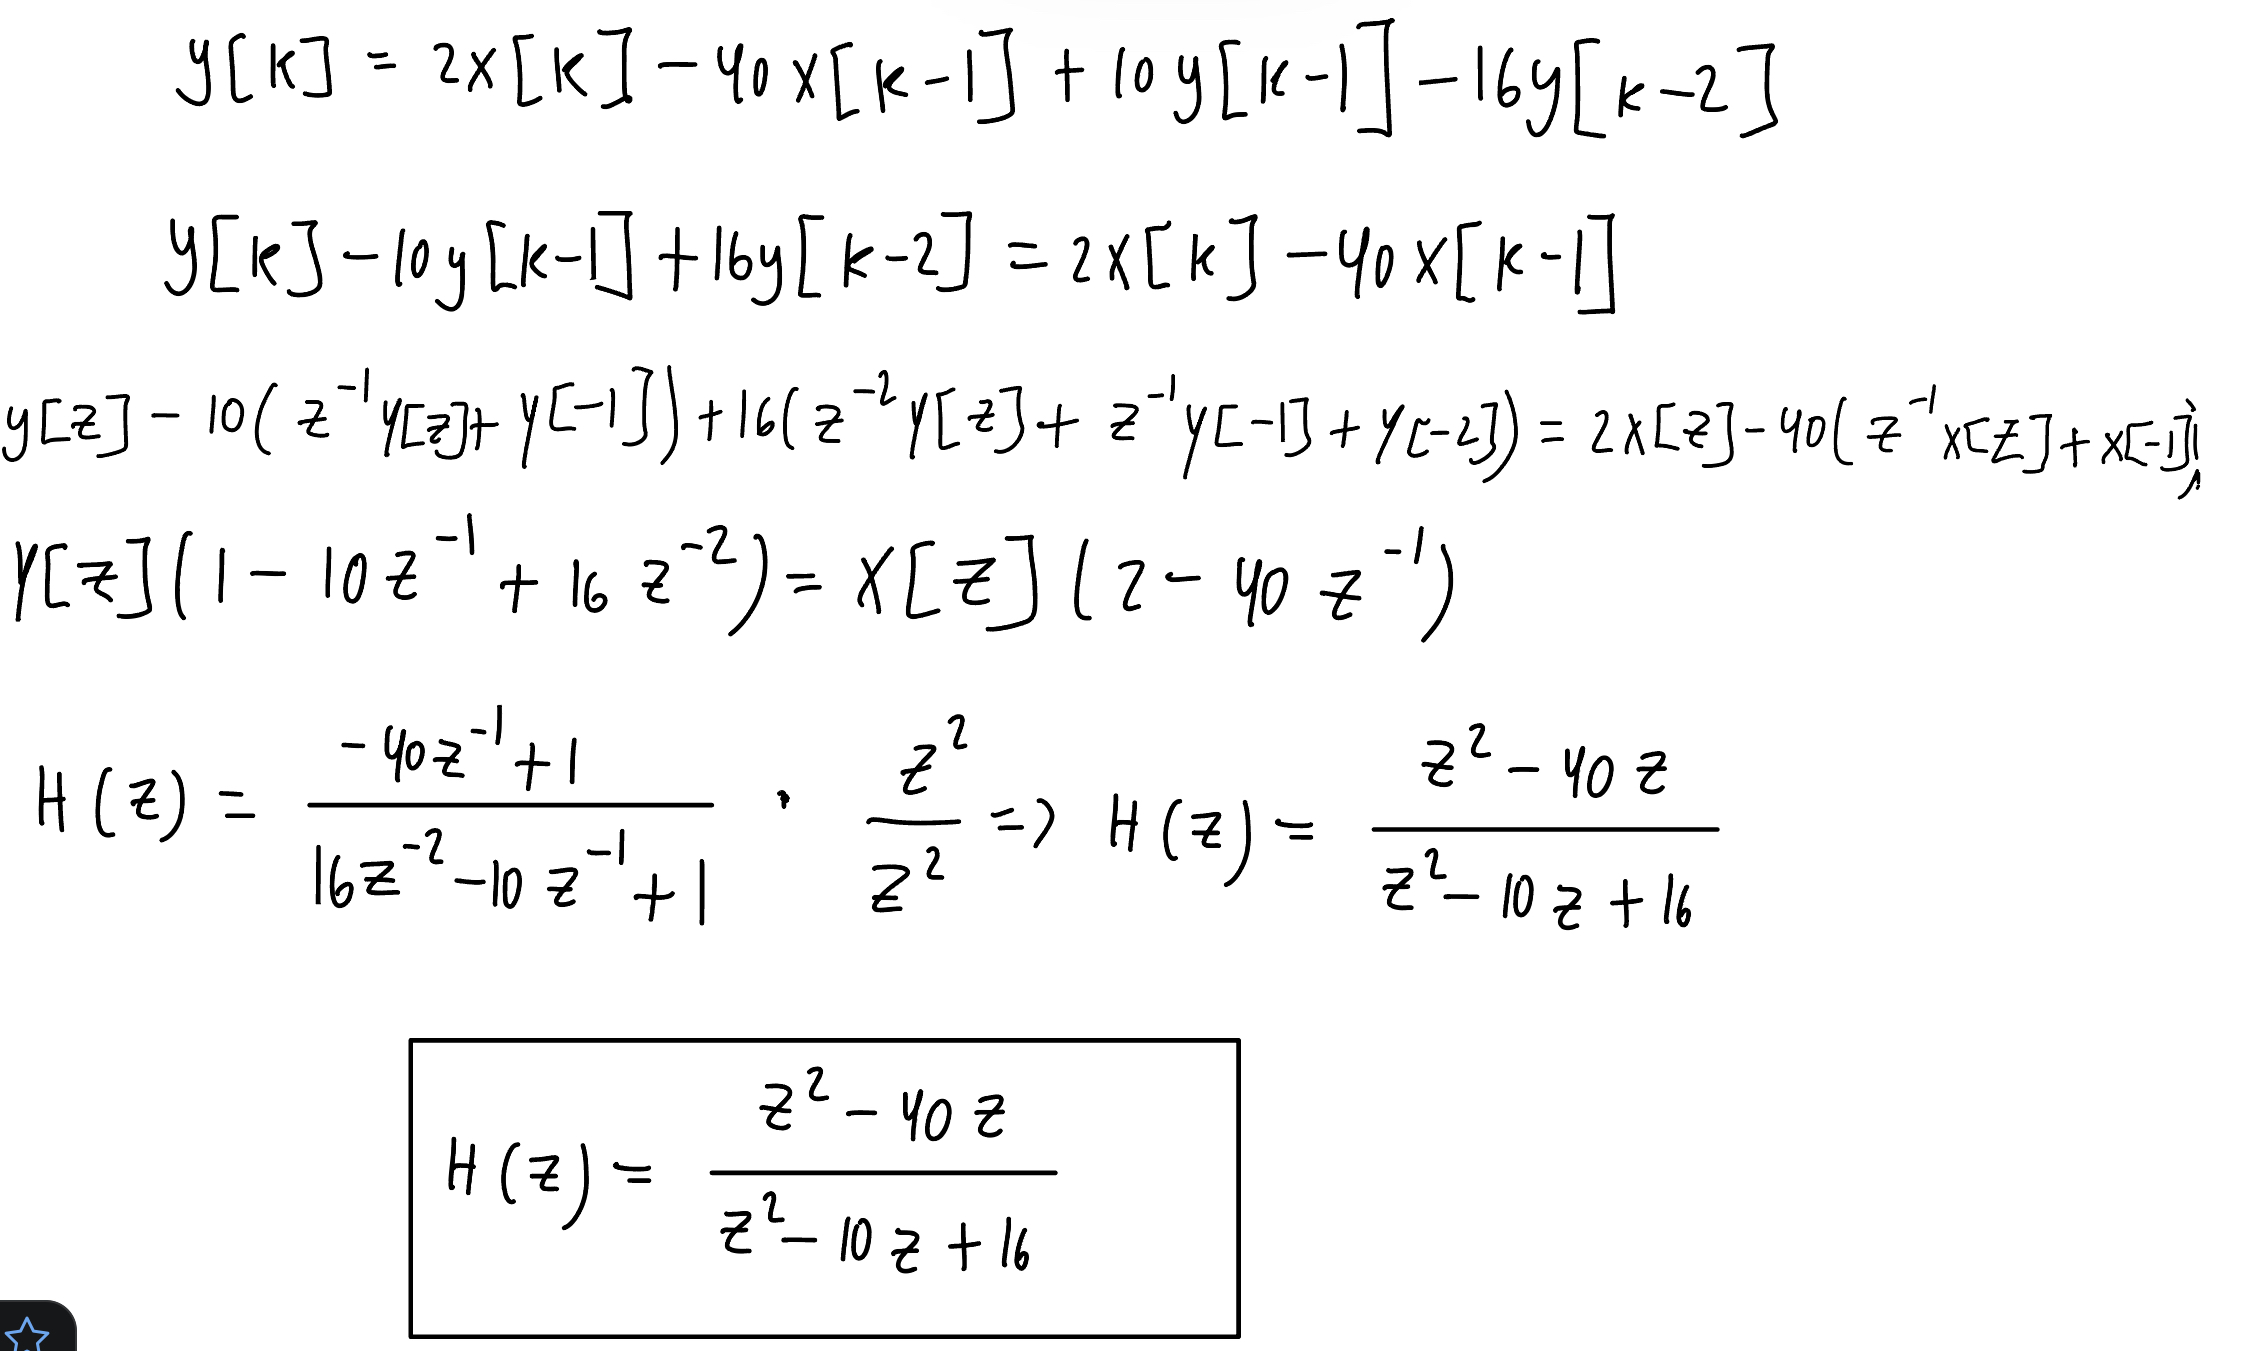
\includegraphics[scale = 0.2]
{txt/Lab11Fig1.jpeg}

Figure 2:

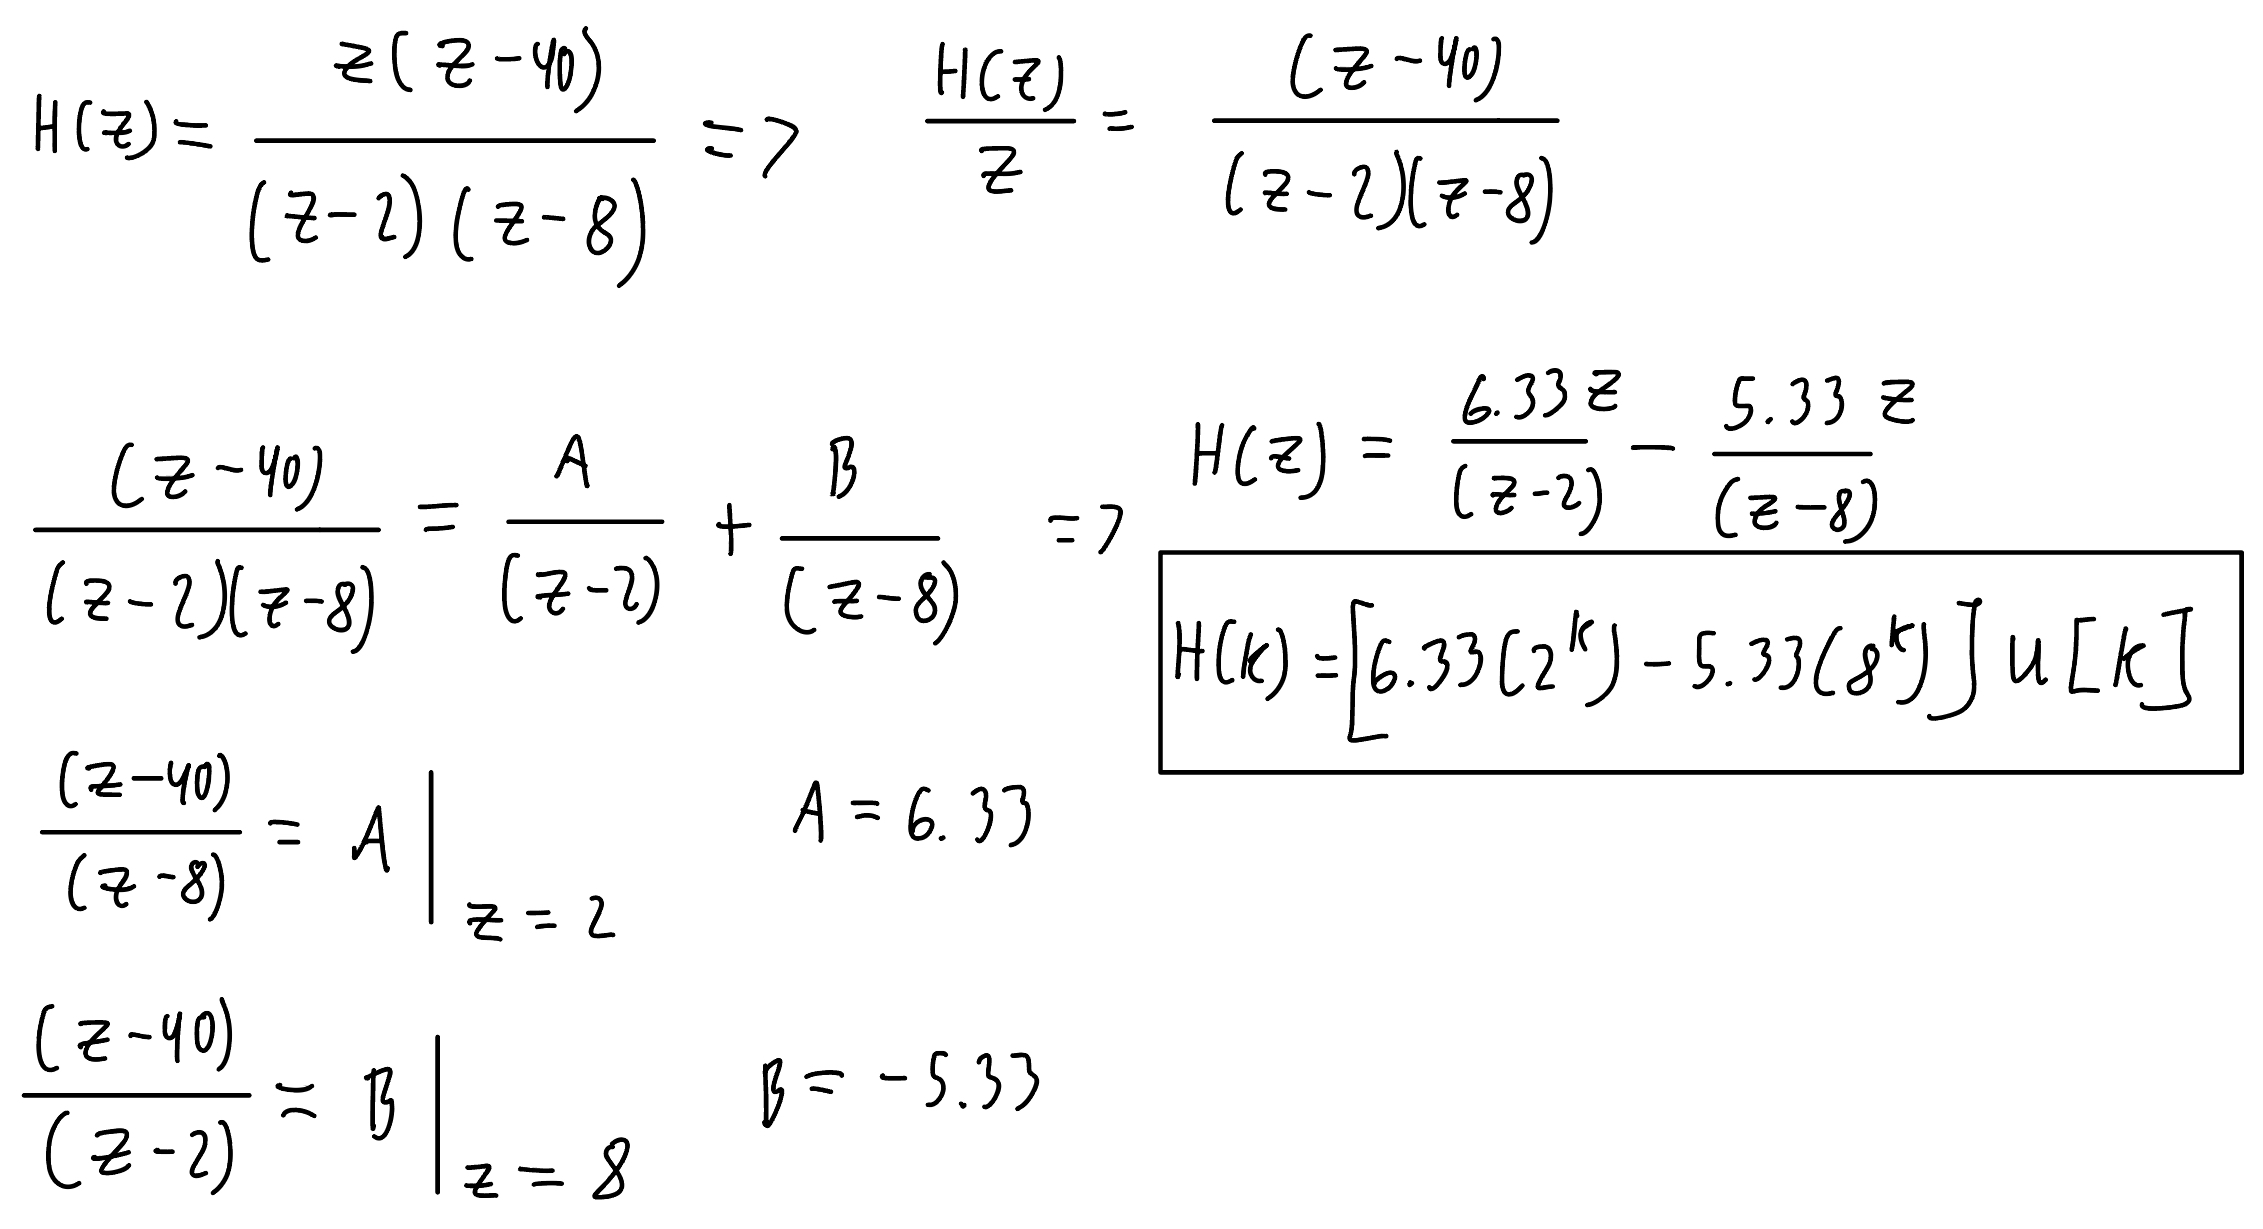
\includegraphics[scale = 0.2]
{txt/Lab11Fig2.jpeg}


Figure 3:

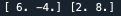
\includegraphics[scale = 1]
{txt/Lab11Fig3.png}

Figure 4:

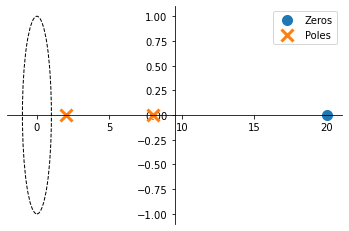
\includegraphics[scale = 0.9]
{txt/Lab11Fig4.png}

Figure 5:

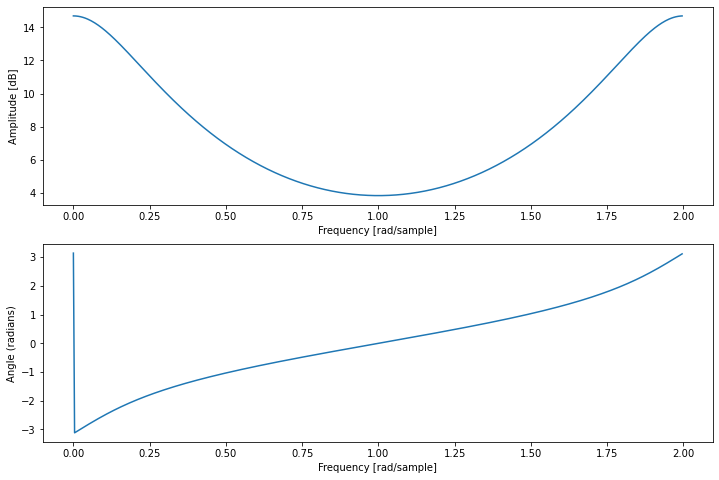
\includegraphics[scale = 0.6]
{txt/Lab11Fig5.png}

\begin{center}
    Conclusion
\end{center}
This lab helped introduce me to some helpful tools for analyzing a discrete system. The scipy.signal.residuez() function can be used to check or preform partial fraction expansion. The zplane() function is useful for finding poles and zeros of a transfer function. The scipy.signal.freqz() function is useful for finding magnitudes and phase responses for a transfer function. 
\end{document}
%%%%%%%%%%%%%%%%%%%%%%%%%%%%%%%%%%%%%%%%

% Copyright Remarks:
%--------------------

% Copyright holder: Vebjørn S. Førde, copyright: CC BY 4.0
% Note: The author of this template is also the copyright holder.

% Below is an explanation of the CC BY 4.0. Additional statements/ 
% clarifications made by the author/copyright holder are marked with *.

% YOU ARE FREE TO:
% Share — copy and redistribute the material in any medium or format
% Adapt — remix, transform, and build upon the material
% for any purpose, even commercially.

% UNDER THE FOLLOWING TERMS:
% Attribution* — You must give appropriate credit, provide a link to the license,
% and indicate if changes were made. You may do so in any reasonable manner, but 
% not in any way that suggests the licensor endorses you or your use.

% *Note: 
% Attribution NOT NEEDED for: 
%       - PDF distibution (like sharing your PDF document)
%       - Use of (dummy)text and images provided in the template (obviously)
%       - Distributing parts of the template, and not the template as a whole
% I am not really concerned with being given credit. As long as you do not 
% claim to have made the template yourself in distributing it further, I have
% no complaints.

% No additional restrictions — You may not apply legal terms or technological 
% measures that legally restrict others from doing anything the license permits.

% NOTICES:
% No warranties are given.

% Disclaimer* (added by copyright holder):
% THE SOFTWARE IS PROVIDED "AS IS", WITHOUT WARRANTY OF ANY KIND, EXPRESS OR
% IMPLIED, INCLUDING BUT NOT LIMITED TO THE WARRANTIES OF MERCHANTABILITY,
% FITNESS FOR A PARTICULAR PURPOSE AND NONINFRINGEMENT. IN NO EVENT SHALL THE
% AUTHORS OR COPYRIGHT HOLDERS BE LIABLE FOR ANY CLAIM, DAMAGES OR OTHER
% LIABILITY, WHETHER IN AN ACTION OF CONTRACT, TORT OR OTHERWISE, ARISING FROM,
% OUT OF OR IN CONNECTION WITH THE SOFTWARE OR THE USE OR OTHER DEALINGS IN THE
% SOFTWARE.

% Read more about CC BY 4.0:
% https://creativecommons.org/licenses/by/4.0/